%Texlive-full Version 3.141592-1.40.3 (Web2C 7.5.6)
%TexStudio Version 2.7.0

\documentclass[a4paper,10pt]{article}
\usepackage[utf8]{inputenc}
\usepackage{graphicx}
\usepackage{subcaption}

\usepackage{lmodern}
\usepackage[a4paper]{geometry}

\usepackage{hyperref}
\usepackage{enumitem}
% \usepackage{nomencl}\makenomenclature

\usepackage{amsmath}
\usepackage{amssymb}
\usepackage{amsthm}

\usepackage{pstricks}
\usepackage{pst-node}
\usepackage{color}
\usepackage[ddmmyyyy]{datetime} 


\newcommand{\E}{\mathbb{E}}

\begin{document}
\begin{titlepage}
%%%%%%%%%%%%%%%%%%%%%%%%%%  LOGO  %%%%%%%%%%%%%%%%%%%%%%%%%%%%%%%%%%%%%%%%%
\begin{center}
\begin{pspicture}(-7,0)(7,2)
%\psline(-7,0)(7,2)
\rput( -4.5,1){\href{www.nakasendoproject.org}{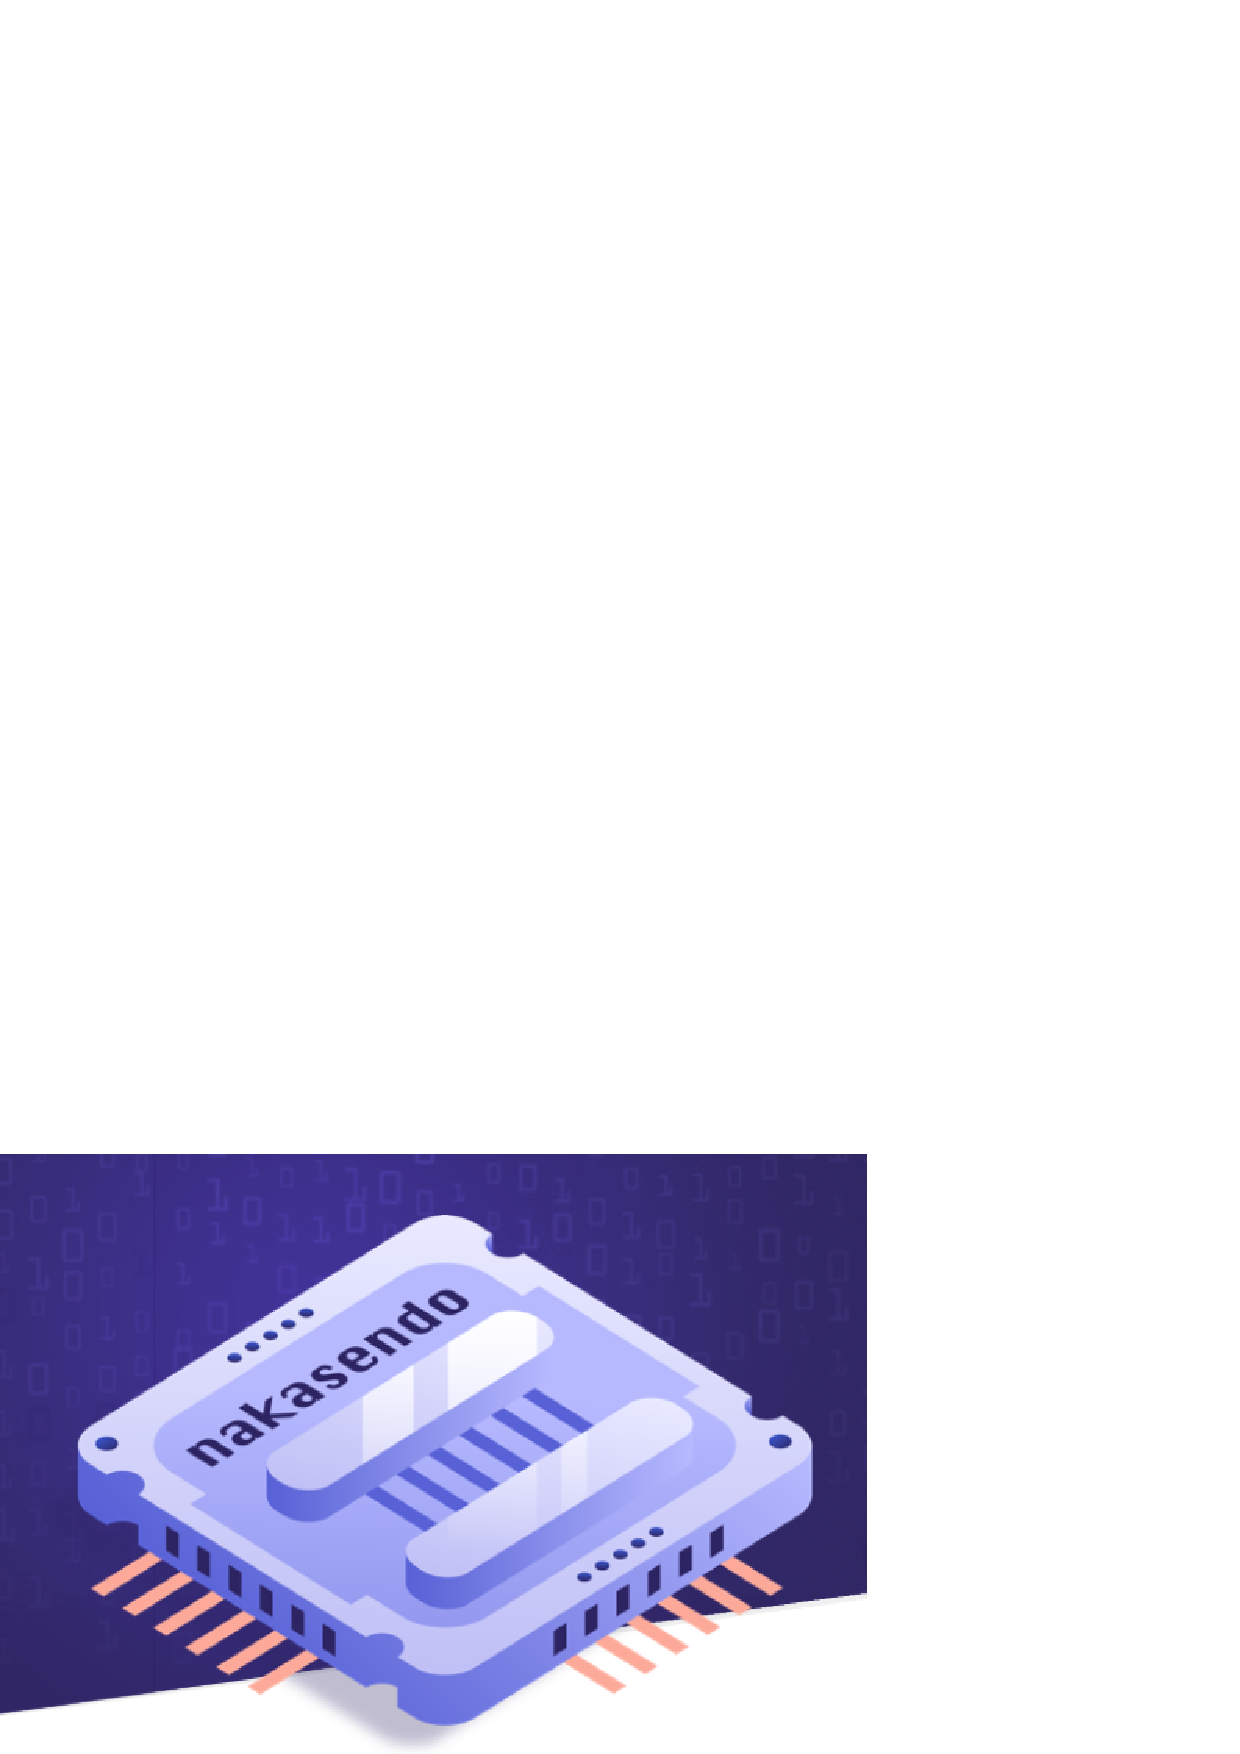
\includegraphics[scale=0.4]{Nakasendo_Logo}}}
\rput(4,2){\href{www.nakasendoproject.org}
	    {	\begin{tabular}{l}
		\resizebox{4cm}{0.6cm}{NAKASENDO}
		\end{tabular}
	    }
}
%\psline(-7,0)(7,2)
\end{pspicture}
\end{center}



%%%%%%%%%%%%%%%%%% DOCUMENT TITLE %%%%%%%%%%%%%%%%%%%%%%%%%
\vspace{2cm}

\begin{center}
\resizebox{14cm}{0.8cm}{Implementation of Threshold Signature}
\end{center}
%%%%%%%%%%%%%%%%%% DOCUMENT TITLE %%%%%%%%%%%%%%%%%%%%%%%%%
\begin{center}
\huge{ Version : \today }
\end{center}


\begin{center}
\href{www.nchain.com}{\LARGE{\textbf{nChain LTD}}}
\end{center}



\vfill
\begin{abstract}
Abstract of implementation of Threshold Signature, with article citing here
\end{abstract}
\end{titlepage}

\tableofcontents
\newpage

%%%%%%%%%%%%%%%%%%%%%%%%%%%%%%%%%%%%%%%
\newpage
%%%%%%%%%%%%%%%%%%%%%%%%%%%%%%%%%%%%%%%%%%%%%%%%%%%%%%%%%%%%%%%%%%%%%%%%%%%%%%%%%%%%%%%%%%%%%%%%%%%%%%%%%%%%%%%%%%%%%%%%%%%%%%%%%%%%%%%%%%%%%%%%%%%%%%%%%%%%
%%%%%%%%%%%%%%%%%%%%%%%%%%%%%%%%%%%%%%%%%%%%%%%%%%%%%%%%%%%%%%%%%%%%%%%%%%%%%%%%%%%%%%%%%%%%%%%%%%%%%%%%%%%%%%%%%%%%%%%%%%%%%%%%%%%%%%%%%%%%%%%%%%%%%%%%%%%%
\section{About Nakasendo project}
Some presentation of the context Nakasendo project within nChain. What is its goals, how it'll help the community

%%%%%%%%%%%%%%%%%%%%%%%%%%%%%%%%%%%%%%%%%%%%%%%%%%%%%%%%%%%%%%%%%%%%%%%%%%%%%%%%%%%%%%%%%%%%%%%%%%%%%%%%%%%%%%%%%%%%%%%%%%%%%%%%%%%%%%%%%%%%%%%%%%%%%%%%%%%%
%%%%%%%%%%%%%%%%%%%%%%%%%%%%%%%%%%%%%%%%%%%%%%%%%%%%%%%%%%%%%%%%%%%%%%%%%%%%%%%%%%%%%%%%%%%%%%%%%%%%%%%%%%%%%%%%%%%%%%%%%%%%%%%%%%%%%%%%%%%%%%%%%%%%%%%%%%%%
\section{Getting started}
Quick tutorial how to build, start by the examples.

%%%%%%%%%%%%%%%%%%%%%%%%%%%%%%%%%%%%%%%%%%%%%%%%%%%%%%%%%%%%%%%%%%%%%%%%%%%%%%%%%%%%%%%%%%%%%%%%%%%%%%%%%%%%%%%%%%%%%%%%%%%%%%%%%%%%%%%%%%%%%%%%%%%%%%%%%%%%
%%%%%%%%%%%%%%%%%%%%%%%%%%%%%%%%%%%%%%%%%%%%%%%%%%%%%%%%%%%%%%%%%%%%%%%%%%%%%%%%%%%%%%%%%%%%%%%%%%%%%%%%%%%%%%%%%%%%%%%%%%%%%%%%%%%%%%%%%%%%%%%%%%%%%%%%%%%%
\section{Threshold Signature implementation}
Inspired by the Shamir's secret sharing algorithm, the threshold signature algorithm is build on polynomial operations on a finite group. The polynomial operations are essentially the fundamental one :
\begin{itemize}
	\item[--] Polynomial evaluation
	\item[--] Polynomial interpolation (Lagrange)
\end{itemize}
The additional \textit{finite group} property simply means \textit{taking the modulo of the final result.} Below are brief explanation of those operations.
\subsection{Mathematical calculation}%%%%%%%%%%%%%%%%%%%%%%%%%%%%%%%%%%%%%%%%%%%%%%%%%%%%%%%%%%%%%%%%%%%%%%%%%%%%%%
\paragraph{Polynomial degree n} is defined as a list of \textbf{n+1} coefficients
\[ 
\textbf{p} \equiv [a_0, a_1 ... , a_n]
\]
that providing any value $x$, the evaluation of the polynomial is 
\[ 
\textbf{p}(x) = a_0 + a_1 x^1 +...+ a_n x^n = \sum^{n}_{i=0} a_i x^i
\]
In our use case, we assume $a_i$ are positives\footnote{Positivity make it easier to manipulate values in finite group???} and $a_0$, $a_n$ are strictly positive\footnote{$a_0$ is the shared secret, so it need to be non zero. $a_n$ need to be non zero to ensure the polynomial is of degree $n$}. Note that the sum and product of two polynomials \textbf{A} and \textbf{B} is a polynomial with
\[
\begin{array}{rcl}
\text{degree } \textbf{A} + \textbf{B} & = & \text{max}(\text{degree }\textbf{A}, \text{degree }\textbf{B}) \\
\text{degree } \textbf{A} \cdot \textbf{B} & = & \text{degree }\textbf{A} + \text{degree }\textbf{B}
\end{array}
\]

\paragraph{Polynomial interpolation} is an other way of defining a polynomial by providing the set of points that the polynomial passes through. The simplified idea is a line (which is a polynomial degree 1) is determined by any two points it passes through. For a polynomial degree \textbf{n}, it is completely determined by providing \textbf{n+1} points :
\[ 
\left[ \begin{array}{c} y_0 \\ x_0 \end{array} \right]
\left[ \begin{array}{c} y_1 \\ x_1 \end{array} \right]
\dots
\left[ \begin{array}{c} y_p \\ x_p \end{array} \right]
\dots
\left[ \begin{array}{c} y_n \\ x_n \end{array} \right]
\]
The evaluation of this polynomial is called Lagrange interpolator\footnote{We implicitly understood $y_p$ is the evaluation of the polynomial $\textbf{p}(x_p)$}, i.e for any value $x$ :
\begin{equation}
\label{eq:interpolation_eq0}
\textbf{L}(x) = \sum^{n}_{p=0} y_p \textbf{b}_p(x) = \sum^{n}_{p=0} \textbf{p}(x_p) \textbf{b}_p(x)
\hspace{2cm}
\textbf{b}_p(x) = \prod_{q \neq p}\frac{x - x_q}{x_p - x_q}
\end{equation}
with $\textbf{b}_p$ is the p-th Lagrangian basis interpolator. Note that the calculation of $\textbf{b}_p(x)$ doesn't require any knowledge of $y_p$ values. It is important to remark this because later we will see the evaluation of those basis Lagrangians can be precalculated without leaking any information, in particular the value $b_p = \textbf{b}_p(0)$. It is also easy to deduce some properties of those polynomials :
\[
\textbf{b}_p(x_p) = 1
\hspace{2cm}
\textbf{b}_p(x_q) = 0
\hspace{2cm}
\textbf{L}(x_i) = y_i
\]
\paragraph{Traditional ECDSA formula} defines the signature calculation :
\begin{equation}
\label{eq:ecdsa_eq0}
s=k^{-1} [ \text{H}(m) + d \cdot r ] \text{ mod } n
\end{equation}
Where :
\begin{itemize}
	\item[-] $n$ is the order of the finite group defined by the elliptic curve
	\item[-] $m$ is the message to be signed
	\item[-] H is hash function. It helps to convert any message to a big number
	\item[-] $k$ is the ephemeral key, randomly generated by each signature process
	\item[-] $d$ is the private key, to be hold \textit{uniquely} by the signer
	\item[-] $(s,r)$ is the calculated signature, with $r$ the $x$-coordinate (modulo $n$) of the public key calculated by the ephemeral key : $r = \| k\otimes\text{G} \|_{x}$
\end{itemize}
In this traditional signing algorithm, a single signer keeping the private key $d$ secret, for each signing process, will generate a random ephemeral key $k$, then calculates the value of $s$ and $r$ as explained above. The signature $(s,r)$ and the signed message $m$ can then be sent over to everyone in order to verify the ownership of the private key $d$.
\paragraph{Shamir's secret sharing} is the fundamental algorithm to start a \textit{threshold cryptosystem}. It is defined by a $(t,n)$-threshold configuration ($t \leq n$), where within a group of $n$ players, it requires at least $t$ of these players to decrypt the cipher text or sign a message. Less than $t$ players will not be able to do anything. The main idea is based on the interpolation of a polynomial degree $t-1$
\[ 
\textbf{p}(x) = a_0 + a_1 x^1 +...+ a_{t-1} x^{t-1} = \sum^{t-1}_{i=0} a_i x^i
\]
where $a_0$ is the hidden secret. A dealer will generate $n$ shared secrets by evaluating the polynomial at $n$ values\footnote{We implicitly understood that each player is labelled by an index $i$ which is known publicly} : $x_i=i$. The dealer then distributes the $n$ shared secrets $\textbf{p}(x_i)=\textbf{p}(i)$ to the corresponding player. When $t$ players regroups together, they provides their label $x_i$ and their corresponding shared secret $\textbf{p}(x_i)$ which make a pack of information :
\[ 
\left[ \begin{array}{c} \textbf{p}(x_0) \\ x_0 \end{array} \right]
\left[ \begin{array}{c} \textbf{p}(x_1) \\ x_1 \end{array} \right]
\dots
\left[ \begin{array}{c} \textbf{p}(x_i) \\ x_i \end{array} \right]
\dots
\left[ \begin{array}{c} \textbf{p}(x_t) \\ x_t \end{array} \right]
\]
That will allow the dealer (or anyone else) calculates the hidden secret $a_0=\textbf{p}(0)$ using the interpolation equation (\ref{eq:interpolation_eq0}).
\subsection{Dealerless ECDSA threshold signature}%%%%%%%%%%%%%%%%%%%%%%%%%%%%%%%%%%%%%%%%%%%%%%%%%%%%%%%%%%%%%%%%%%%%%%%%%%%%%%
\paragraph{} The dealerless ECDSA threshold signature algorithm uses the mathematical building blocks explained above. It essentially rebuilds the signature equation (\ref{eq:ecdsa_eq0}) with the shared secret splitting processes to hide the secret $k$ and $d$. In order to understand the algorithm, one should be familiar with the idea $k$ and $d$ numbers are split to shared secret through polynomials \textbf{k} and \textbf{d}. Further more, to protect the secret $k$, a binding value $\alpha$ (with corresponding polynomial {\boldmath$\alpha$}) is introduced. Pairing with $k$, it give the value of $k^{-1}$ by $k^{-1} = (k\alpha)^{-1}\alpha$. Note that equation (\ref{eq:ecdsa_eq0}) doesn't require $k$ but $k^{-1}$, it means users does not need to broadcast their shared secrets of $k$, but they send their shared secrets of $(k\alpha)^{-1}$ and $\alpha$. The additional polynomial {\boldmath$\alpha$} requires defining a polynomial product \textbf{k}{\boldmath$\alpha$} which double the polynomial degree space ($2t-2$). This multiplication (and $k^{-1}d$) requires our threshold signature scheme the participation of at least $2t-1$ of $n$ players to perform signing process.
\paragraph{} In order to make the best understanding of the following explanation , it is useful to define a few conventions :
\begin{itemize}
	\item[-] All players in the global group are indexed by an integer from $1$ to $n$. Their index (label) are supposed to be known by everyone. When we talk about player $i$, we talk about their indentification $i$ and their corresponding label ($x$-coordinate $x_i=i$).
	\item[-] When we talk about a secret represented by a letter, it has the corresponding polynomial represented by the bold letter, and the evaluation of the polynomial is represented by the indexed letter. For example the secret $d$ use the polynomial \textbf{d} to calculate the shared secret $d_i=\textbf{d}(i)$ which belong to the player $i$.
    \item[-] As there usage of polynomial product which increase the polynomial degree, we define two group of players $\pi\subseteq\Pi$ where $\Pi$ is the group of $2t-1$ players and its subgroup $\pi$ of $t$ players. They are able to build the interpolation for polynomial of degree $2t-2$ and respectively $t-1$.
    \item[-] In usage of the binding value $\alpha$, it is easier to rewrite the signature equation to 
    \begin{equation}
    \label{eq:ecdsa_eq1}
    s=(k\alpha)^{-1} \alpha [ \text{H}(m) + d \cdot r ] \text{ mod } n
    \end{equation}
\end{itemize}
The dealerless ECDSA threshold signature algorithm is split into three main steps, each calculates part of the expression (\ref{eq:ecdsa_eq1}) :
\begin{itemize}
	\item[-] Calculation of $r$
	\item[-] Calculation of $(k\alpha)^{-1}$
	\item[-] Calculation of $s$
\end{itemize}
From the following explanation, the modulo operation is omitted to simplify the expressions. Users has to remember to take modulo $n$ at every step they have the result of a calculation\footnote{$n$ is the order of the elliptic curve group}.
\paragraph{Step 0} Each player $i$ in the group $\Pi$ has (randomly generated) their private polynomial\footnote{Except the zero-degree coefficient for polynomial \textbf{d} that should be kept permanantly because it form the private key $d$} \textbf{d}, \textbf{k} and {\boldmath$\alpha$}. They evaluate their polynomials at their label $x_i=i$ to get the shared secrets $d_i$, $k_i$ and $\alpha_i$. Using equation (\ref{eq:interpolation_eq0}), they can also precalculate the interpolation weight of every one which is the evaluation of the Lagrangian basis polynomial at zero : 
\[
B_{i} = \prod_{j \neq i \in \Pi}\frac{-j}{i - j}
\hspace{2cm}
b_{i} = \prod_{j \neq i \in \pi}\frac{-j}{i - j}
\]
\paragraph{Calculation of $r$} : Each player $i$ in the group $\Pi$ calculate  their share $k_i \cdot\textbf{G}$ , broadcast to everyone. Once the broadcast finishes, everyone randomly pick a subgroup $\pi\subseteq\Pi$ calculate the interpolation weight for this subgroup $b_i$, sum up then take the $x$-coordinate to get
\[
r=\|\textbf{k}(0)\cdot\textbf{G}\|_{x}=\|\sum_{i\in\pi} k_ib_i\cdot\textbf{G}\|_{x}
\]
After this step, everyone has $r$
\paragraph{Calculation of $(k\alpha)^{-1}$} : Each player $i$ in the group $\Pi$ calculate  their share $k_i\alpha_i B_i$, broadcast to everyone. Once the broadcast finishes, everyone sum up all shares, calculate the inverse to get 
\[
(k\alpha)^{-1} =\frac{1}{\textbf{k{\boldmath$\alpha$}}(0)}=(\sum_{i\in\Pi} k_i \alpha_i B_i)^{-1}
\]
After this step, everyone has $(k\alpha)^{-1}$
\paragraph{Calculation of $s$} : Each player $i$ in the group $\Pi$ calculate their share $(k\alpha)^{-1} \alpha_i [ \text{H}(m) + d_i \cdot r ]B_i$, broadcast to everyone. Once the broadcast finishes, everyone sum up all to get
\[
s=\textbf{s}(0)=\sum_{i\in\Pi}(k\alpha)^{-1} \alpha_i [ \text{H}(m) + d_i \cdot r ]B_i
\]
\subsection{Protocol}%%%%%%%%%%%%%%%%%%%%%%%%%%%%%%%%%%%%%%%%%%%%%%%%%%%%%%%%%%%%%%%%%%%%%%%%%%%%%%
All descripstion of protocol
\subsection{Examples and demo}%%%%%%%%%%%%%%%%%%%%%%%%%%%%%%%%%%%%%%%%%%%%%%%%%%%%%%%%%%%%%%%%%%%%%%%%%%%%%%
Where to find example and demo/ testcase

\end{document}